\documentclass[12pt,a4paper]{report}

% ============================================================================
% PACKAGES
% ============================================================================
\usepackage[utf8]{inputenc}
\usepackage[T1]{fontenc}
\usepackage{lmodern}
\usepackage[margin=1in]{geometry}
\usepackage{graphicx}
\usepackage{xcolor}
\usepackage{hyperref}
\usepackage{tikz}
\usepackage{longtable}
\usepackage{booktabs}
\usepackage{fancyhdr}
\usepackage{titlesec}
\usepackage{listings}
\usepackage{enumitem}

% TikZ Libraries
\usetikzlibrary{shapes.geometric, arrows.meta, positioning, fit, backgrounds, matrix}

% ============================================================================
% COLORS
% ============================================================================
\definecolor{primaryblue}{RGB}{26, 54, 93}
\definecolor{secondaryblue}{RGB}{59, 130, 246}
\definecolor{accentgreen}{RGB}{34, 197, 94}
\definecolor{warningorange}{RGB}{249, 115, 22}
\definecolor{dangerred}{RGB}{239, 68, 68}
\definecolor{lightgray}{RGB}{243, 244, 246}
\definecolor{darkgray}{RGB}{75, 85, 99}

% ============================================================================
% HYPERREF SETUP
% ============================================================================
\hypersetup{
    colorlinks=true,
    linkcolor=primaryblue,
    urlcolor=secondaryblue,
    pdftitle={EduX - Attendance Management Guide},
    pdfauthor={EduX Development Team},
}

% ============================================================================
% HEADER/FOOTER
% ============================================================================
\pagestyle{fancy}
\fancyhf{}
\fancyhead[L]{\textcolor{darkgray}{\small EduX School Management System}}
\fancyhead[R]{\textcolor{darkgray}{\small Attendance Guide}}
\fancyfoot[C]{\textcolor{darkgray}{\thepage}}
\renewcommand{\headrulewidth}{0.4pt}

% ============================================================================
% TITLE FORMATTING
% ============================================================================
\titleformat{\chapter}[display]
  {\normalfont\huge\bfseries\color{primaryblue}}
  {\chaptertitlename\ \thechapter}{20pt}{\Huge}

\titleformat{\section}
  {\normalfont\Large\bfseries\color{primaryblue}}
  {\thesection}{1em}{}

\titleformat{\subsection}
  {\normalfont\large\bfseries\color{secondaryblue}}
  {\thesubsection}{1em}{}

% ============================================================================
% DOCUMENT
% ============================================================================
\begin{document}

% ----------------------------------------------------------------------------
% TITLE PAGE
% ----------------------------------------------------------------------------
\begin{titlepage}
    \centering
    \vspace*{2cm}
    
    {\Huge\bfseries\textcolor{primaryblue}{EduX}\par}
    \vspace{0.5cm}
    {\Large\textcolor{secondaryblue}{School Management System}\par}
    
    \vspace{2cm}
    
    
\begin{tikzpicture}
        \node[draw=primaryblue, line width=2pt, rounded corners=10pt, 
              minimum width=8cm, minimum height=3cm, fill=lightgray] 
              {\Huge\bfseries\textcolor{primaryblue}{Attendance Management}};
    \end{tikzpicture}
    
    \vfill
    
    {\large\textcolor{darkgray}{Version 1.0}\par}
    {\large\textcolor{darkgray}{\today}\par}
\end{titlepage}

\tableofcontents
\newpage

% ============================================================================
% CHAPTER 1: OVERVIEW
% ============================================================================
\chapter{Attendance Overview}

\section{Introduction}

The Attendance module tracks daily presence of students and staff. It provides real-time insights, alerts for low attendance, and comprehensive reporting.

\section{Attendance Statuses}

\begin{center}
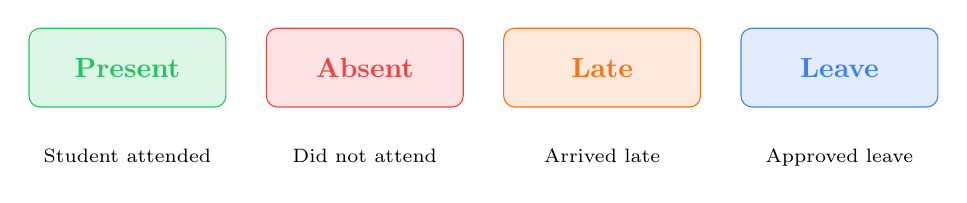
\begin{tikzpicture}[
    status/.style={draw=#1, rounded corners, minimum width=2.5cm, 
                   minimum height=1cm, fill=#1!15, font=\bfseries, text=#1}
]
    \node[status=accentgreen] (present) at (0,0) {Present};
    \node[status=dangerred, right=0.5cm of present] (absent) {Absent};
    \node[status=warningorange, right=0.5cm of absent] (late) {Late};
    \node[status=secondaryblue, right=0.5cm of late] (leave) {Leave};
    
    \node[below=0.4cm of present, font=\scriptsize, text width=2.3cm, align=center] 
        {Student attended};
    \node[below=0.4cm of absent, font=\scriptsize, text width=2.3cm, align=center] 
        {Did not attend};
    \node[below=0.4cm of late, font=\scriptsize, text width=2.3cm, align=center] 
        {Arrived late};
    \node[below=0.4cm of leave, font=\scriptsize, text width=2.3cm, align=center] 
        {Approved leave};
\end{tikzpicture}
\end{center}

\section{Daily Workflow}

\begin{center}
\begin{tikzpicture}[
    node distance=1cm,
    step/.style={draw=secondaryblue, rounded corners, minimum width=4.5cm, 
                 minimum height=1cm, fill=lightgray, align=center, font=\small},
    arrow/.style={-{Stealth}, thick, secondaryblue}
]
    \node[step] (s1) {Select Date \& Class};
    \node[step, below=of s1] (s2) {Load Student List};
    \node[step, below=of s2] (s3) {Mark Attendance};
    \node[step, below=of s3] (s4) {Add Remarks (Optional)};
    \node[step, below=of s4] (s5) {Save Attendance};
    
    \draw[arrow] (s1) -- (s2);
    \draw[arrow] (s2) -- (s3);
    \draw[arrow] (s3) -- (s4);
    \draw[arrow] (s4) -- (s5);
\end{tikzpicture}
\end{center}

% ============================================================================
% CHAPTER 2: MARKING ATTENDANCE
% ============================================================================
\chapter{Marking Student Attendance}

\section{Accessing Attendance}

Navigate to \texttt{Attendance} from the sidebar or use keyboard shortcut \texttt{Ctrl + A}.

\section{Select Class and Date}

\begin{enumerate}[leftmargin=*]
    \item Select the \textbf{Class} from dropdown
    \item Select the \textbf{Section} (if applicable)
    \item Choose the \textbf{Date} (defaults to today)
    \item Click \textbf{Load Students}
\end{enumerate}

\section{Mark Individual Students}

The attendance grid shows all enrolled students:

\begin{center}
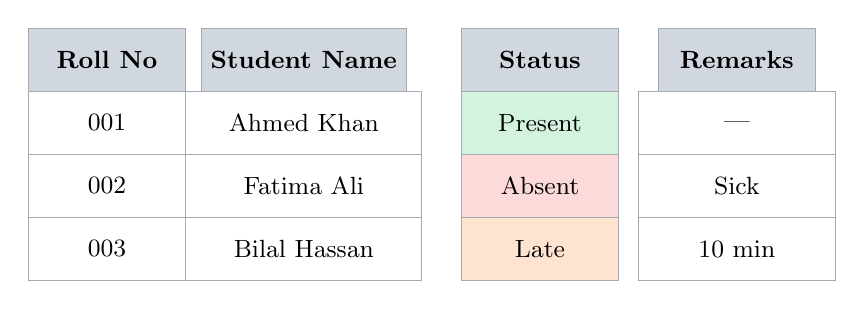
\begin{tikzpicture}[
    cell/.style={minimum width=2cm, minimum height=0.8cm, draw=darkgray!50, 
                 font=\small},
    header/.style={cell, fill=primaryblue!20, font=\small\bfseries}
]
    % Headers
    \node[header] at (0,0) {Roll No};
    \node[header] at (2.5,0) {Student Name};
    \node[header] at (5.5,0) {Status};
    \node[header] at (8,0) {Remarks};
    
    % Row 1
    \node[cell] at (0,-0.8) {001};
    \node[cell, minimum width=3cm] at (2.5,-0.8) {Ahmed Khan};
    \node[cell, fill=accentgreen!20] at (5.5,-0.8) {Present};
    \node[cell, minimum width=2.5cm] at (8,-0.8) {---};
    
    % Row 2
    \node[cell] at (0,-1.6) {002};
    \node[cell, minimum width=3cm] at (2.5,-1.6) {Fatima Ali};
    \node[cell, fill=dangerred!20] at (5.5,-1.6) {Absent};
    \node[cell, minimum width=2.5cm] at (8,-1.6) {Sick};
    
    % Row 3
    \node[cell] at (0,-2.4) {003};
    \node[cell, minimum width=3cm] at (2.5,-2.4) {Bilal Hassan};
    \node[cell, fill=warningorange!20] at (5.5,-2.4) {Late};
    \node[cell, minimum width=2.5cm] at (8,-2.4) {10 min};
\end{tikzpicture}
\end{center}

\section{Quick Actions}

\begin{itemize}[leftmargin=*]
    \item \textbf{Mark All Present} -- Sets all students as present
    \item \textbf{Mark All Absent} -- Sets all students as absent
    \item \textbf{Copy from Yesterday} -- Copies previous day's attendance
    \item \textbf{Save} -- Saves current attendance
\end{itemize}

\section{Adding Remarks}

Click on the remarks field to add notes:
\begin{itemize}[leftmargin=*]
    \item Reason for absence (sick, family emergency)
    \item Late arrival time
    \item Early departure
    \item Any special notes
\end{itemize}

% ============================================================================
% CHAPTER 3: VIEWING ATTENDANCE
% ============================================================================
\chapter{Viewing Attendance Records}

\section{Daily View}

Shows attendance for all students on a specific date:
\begin{itemize}[leftmargin=*]
    \item Summary: Present / Absent / Late / Leave counts
    \item Percentage attendance for the day
    \item Color-coded status indicators
\end{itemize}

\section{Student History}

View individual student attendance:
\begin{enumerate}[leftmargin=*]
    \item Go to \texttt{Students} $\rightarrow$ Select Student
    \item Click \texttt{View Attendance}
    \item Select date range
    \item View calendar or list view
\end{enumerate}

\section{Class Summary}

\begin{center}
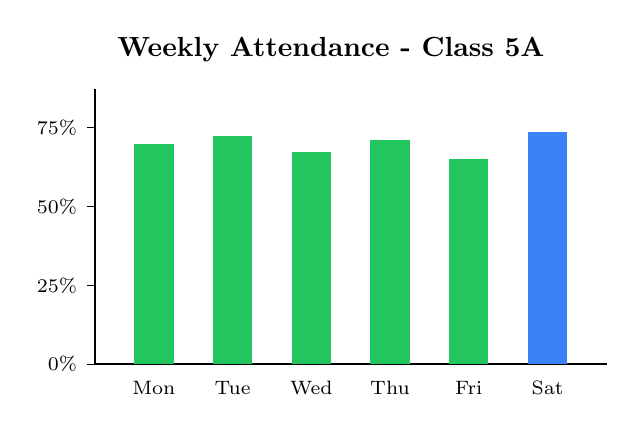
\begin{tikzpicture}[
    bar/.style={minimum width=0.5cm, draw=none},
]
    % Chart title
    \node[font=\bfseries] at (3,4) {Weekly Attendance - Class 5A};
    
    % Y-axis
    \draw[thick] (0,0) -- (0,3.5);
    \foreach \y/\label in {0/0\%, 1/25\%, 2/50\%, 3/75\%} {
        \draw (0,\y) -- (-0.1,\y) node[left, font=\scriptsize] {\label};
    }
    
    % X-axis
    \draw[thick] (0,0) -- (6.5,0);
    
    % Bars
    \fill[accentgreen] (0.5,0) rectangle (1,2.8);
    \fill[accentgreen] (1.5,0) rectangle (2,2.9);
    \fill[accentgreen] (2.5,0) rectangle (3,2.7);
    \fill[accentgreen] (3.5,0) rectangle (4,2.85);
    \fill[accentgreen] (4.5,0) rectangle (5,2.6);
    \fill[secondaryblue] (5.5,0) rectangle (6,2.95);
    
    % Labels
    \node[font=\scriptsize] at (0.75,-0.3) {Mon};
    \node[font=\scriptsize] at (1.75,-0.3) {Tue};
    \node[font=\scriptsize] at (2.75,-0.3) {Wed};
    \node[font=\scriptsize] at (3.75,-0.3) {Thu};
    \node[font=\scriptsize] at (4.75,-0.3) {Fri};
    \node[font=\scriptsize] at (5.75,-0.3) {Sat};
\end{tikzpicture}
\end{center}

% ============================================================================
% CHAPTER 4: ATTENDANCE ALERTS
% ============================================================================
\chapter{Attendance Alerts}

\section{Low Attendance Alerts}

System automatically generates alerts for:
\begin{itemize}[leftmargin=*]
    \item Students with attendance below threshold (default: 75\%)
    \item Consecutive absences (default: 3 days)
    \item Unusual patterns (sudden drops)
\end{itemize}

\section{Alert Configuration}

Configure in \texttt{Settings} $\rightarrow$ \texttt{Attendance Settings}:

\begin{longtable}{@{}p{5cm}p{3cm}p{5cm}@{}}
\toprule
\textbf{Setting} & \textbf{Default} & \textbf{Description} \\
\midrule
\endhead
Minimum Attendance \% & 75\% & Alert threshold \\
Consecutive Absences & 3 days & Days before alert \\
Alert Recipients & Admin & Who receives alerts \\
\bottomrule
\end{longtable}

\section{Viewing Alerts}

\begin{center}
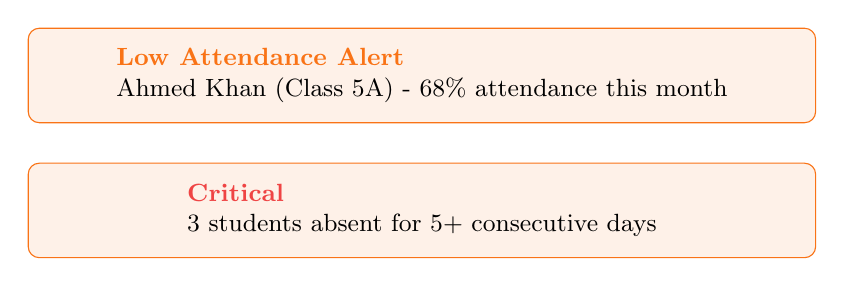
\begin{tikzpicture}[
    alert/.style={draw=warningorange, rounded corners, minimum width=10cm, 
                  minimum height=1.2cm, fill=warningorange!10, align=left, 
                  font=\small}
]
    \node[alert] (a1) at (0,0) {
        \textcolor{warningorange}{\textbf{Low Attendance Alert}}\\
        Ahmed Khan (Class 5A) - 68\% attendance this month
    };
    \node[alert, below=0.5cm of a1] (a2) {
        \textcolor{dangerred}{\textbf{Critical}}\\
        3 students absent for 5+ consecutive days
    };
\end{tikzpicture}
\end{center}

% ============================================================================
% CHAPTER 5: REPORTS
% ============================================================================
\chapter{Attendance Reports}

\section{Available Reports}

\begin{longtable}{@{}p{4cm}p{9cm}@{}}
\toprule
\textbf{Report} & \textbf{Description} \\
\midrule
\endhead
Daily Report & Summary for a specific date \\
Weekly Report & Week-wise attendance summary \\
Monthly Report & Month-wise with trends \\
Student Report & Individual student history \\
Class Report & Class-wise statistics \\
Defaulters Report & Students below threshold \\
\bottomrule
\end{longtable}

\section{Exporting Reports}

\begin{enumerate}[leftmargin=*]
    \item Go to \texttt{Attendance} $\rightarrow$ \texttt{Reports}
    \item Select report type
    \item Choose date range and filters
    \item Select format: \textbf{PDF} or \textbf{Excel}
    \item Click \textbf{Export}
\end{enumerate}

\section{Report Contents}

PDF reports include:
\begin{itemize}[leftmargin=*]
    \item School header with logo
    \item Date range and filters applied
    \item Summary statistics
    \item Detailed records table
    \item Signature lines for verification
\end{itemize}

% ============================================================================
% CHAPTER 6: STAFF ATTENDANCE
% ============================================================================
\chapter{Staff Attendance}

\section{Overview}

Staff attendance includes additional features:
\begin{itemize}[leftmargin=*]
    \item Check-in and check-out times
    \item Half-day tracking
    \item Leave integration
\end{itemize}

\section{Staff Attendance Statuses}

\begin{center}
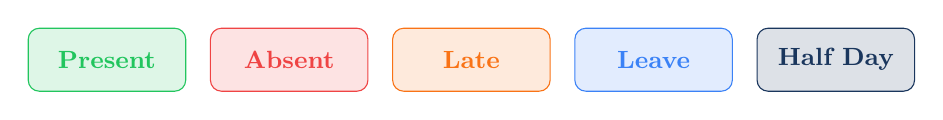
\begin{tikzpicture}[
    status/.style={draw=#1, rounded corners, minimum width=2cm, 
                   minimum height=0.8cm, fill=#1!15, font=\small\bfseries, text=#1}
]
    \node[status=accentgreen] (present) at (0,0) {Present};
    \node[status=dangerred, right=0.3cm of present] (absent) {Absent};
    \node[status=warningorange, right=0.3cm of absent] (late) {Late};
    \node[status=secondaryblue, right=0.3cm of late] (leave) {Leave};
    \node[status=primaryblue, right=0.3cm of leave] (half) {Half Day};
\end{tikzpicture}
\end{center}

\section{Recording Staff Attendance}

\begin{enumerate}[leftmargin=*]
    \item Navigate to \texttt{Staff} $\rightarrow$ \texttt{Attendance}
    \item Select date
    \item Mark status for each staff member
    \item Enter check-in/check-out times
    \item Save attendance
\end{enumerate}

\section{Leave Integration}

When a staff member has approved leave:
\begin{itemize}[leftmargin=*]
    \item Attendance automatically marked as ``Leave''
    \item Cannot be changed unless leave is cancelled
    \item Shows leave type (Sick, Casual, etc.)
\end{itemize}

\end{document}
